\chapter{Východzia situácia}\label{chap:intro} 

V tejto úvodnej kapitole by som vás chcel trochu oboznámiť s mojou bakalárkou a poukázať na moju východziu situáciu. Ďalej tiež platformy na ktorých beží a prečo. 
\section{Vysvetlenie názvu} 
Moja bakalárka sa volá \uv{Optimalizácia obchodovacieho algoritmu na vysoko volatilných komoditných burzách}. Najprv by som tento názov rozobral a podrobne vysvetlil, čo to znamená. 
\subsection{Optimalizácia obchodného algoritmu} 
Vyvíjame algoritmus, ktorý bude vedieť sám obchodovať. Mojou úlohou bude tento algoritmus testovať a následne optimalizovať aby podával čo najlepšie výsledky. 
\subsection{Vysoko volatilných} 
Volatilita\cite{Volatilita} je kolísanie. Miera neistoty. A investíciám je vlastná. Platí, že čím vyššie výnosy, tým vyššia volatilita. Z toho vychádza aj pravidlo investičného horizontu, ktorý je pri rizikovejších – teda volatilnejších – aktívach dlhší. Prečo hľadáme  vysoko volatilné burzy ukážem na príklade neskôr. 
\subsection{Komoditných burzách} 
Náš algoritmus bude pracovať na komoditných burzách, konkrétne na burzách pseudo-mien  hlavne bitcoin. 

\section{Prečo volatilných?} 
V tejto časti sa zameriam na okrajové burzy, ktoré sú špecifické svojou vysokou volatilitou 
a ukážeme výhody a nevýhody okrajových búrz. Nakoniec zhrnieme, prečo nám vyhovujú práve okrajové burzy. 
\subsection{Výhody} 
\subsubsection{Vysoká volatilita} 
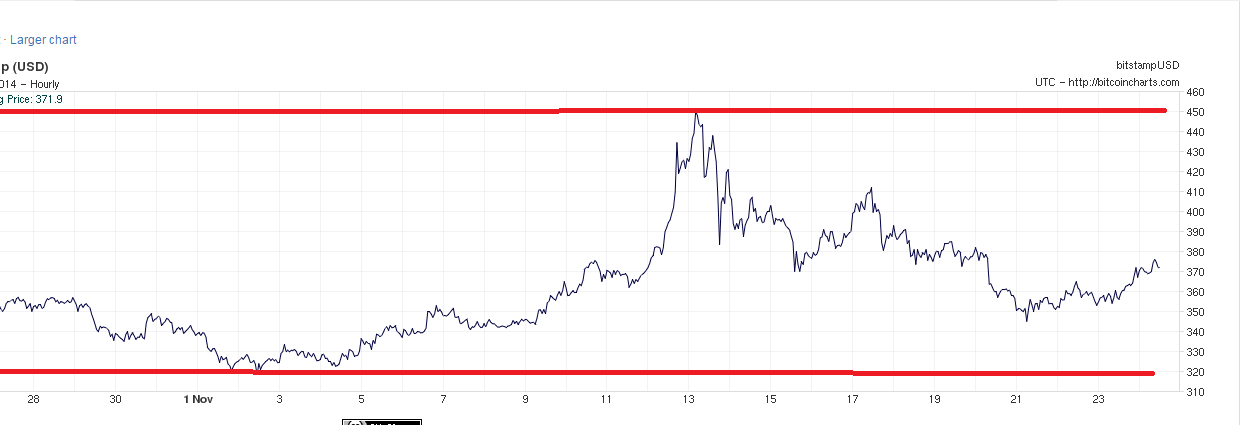
\includegraphics[width=1\textwidth]{obr} 
Toto je príklad, keď pozeráme na vysoko volatilnú burzu, ktorou je bitcoin a USD. Možný zisk sa pohybuje až na úrovni 37,5 percenta, keď nerátame poplatky. V prvom obrázku je jeden dielik 10 dolárov. 
\\ 
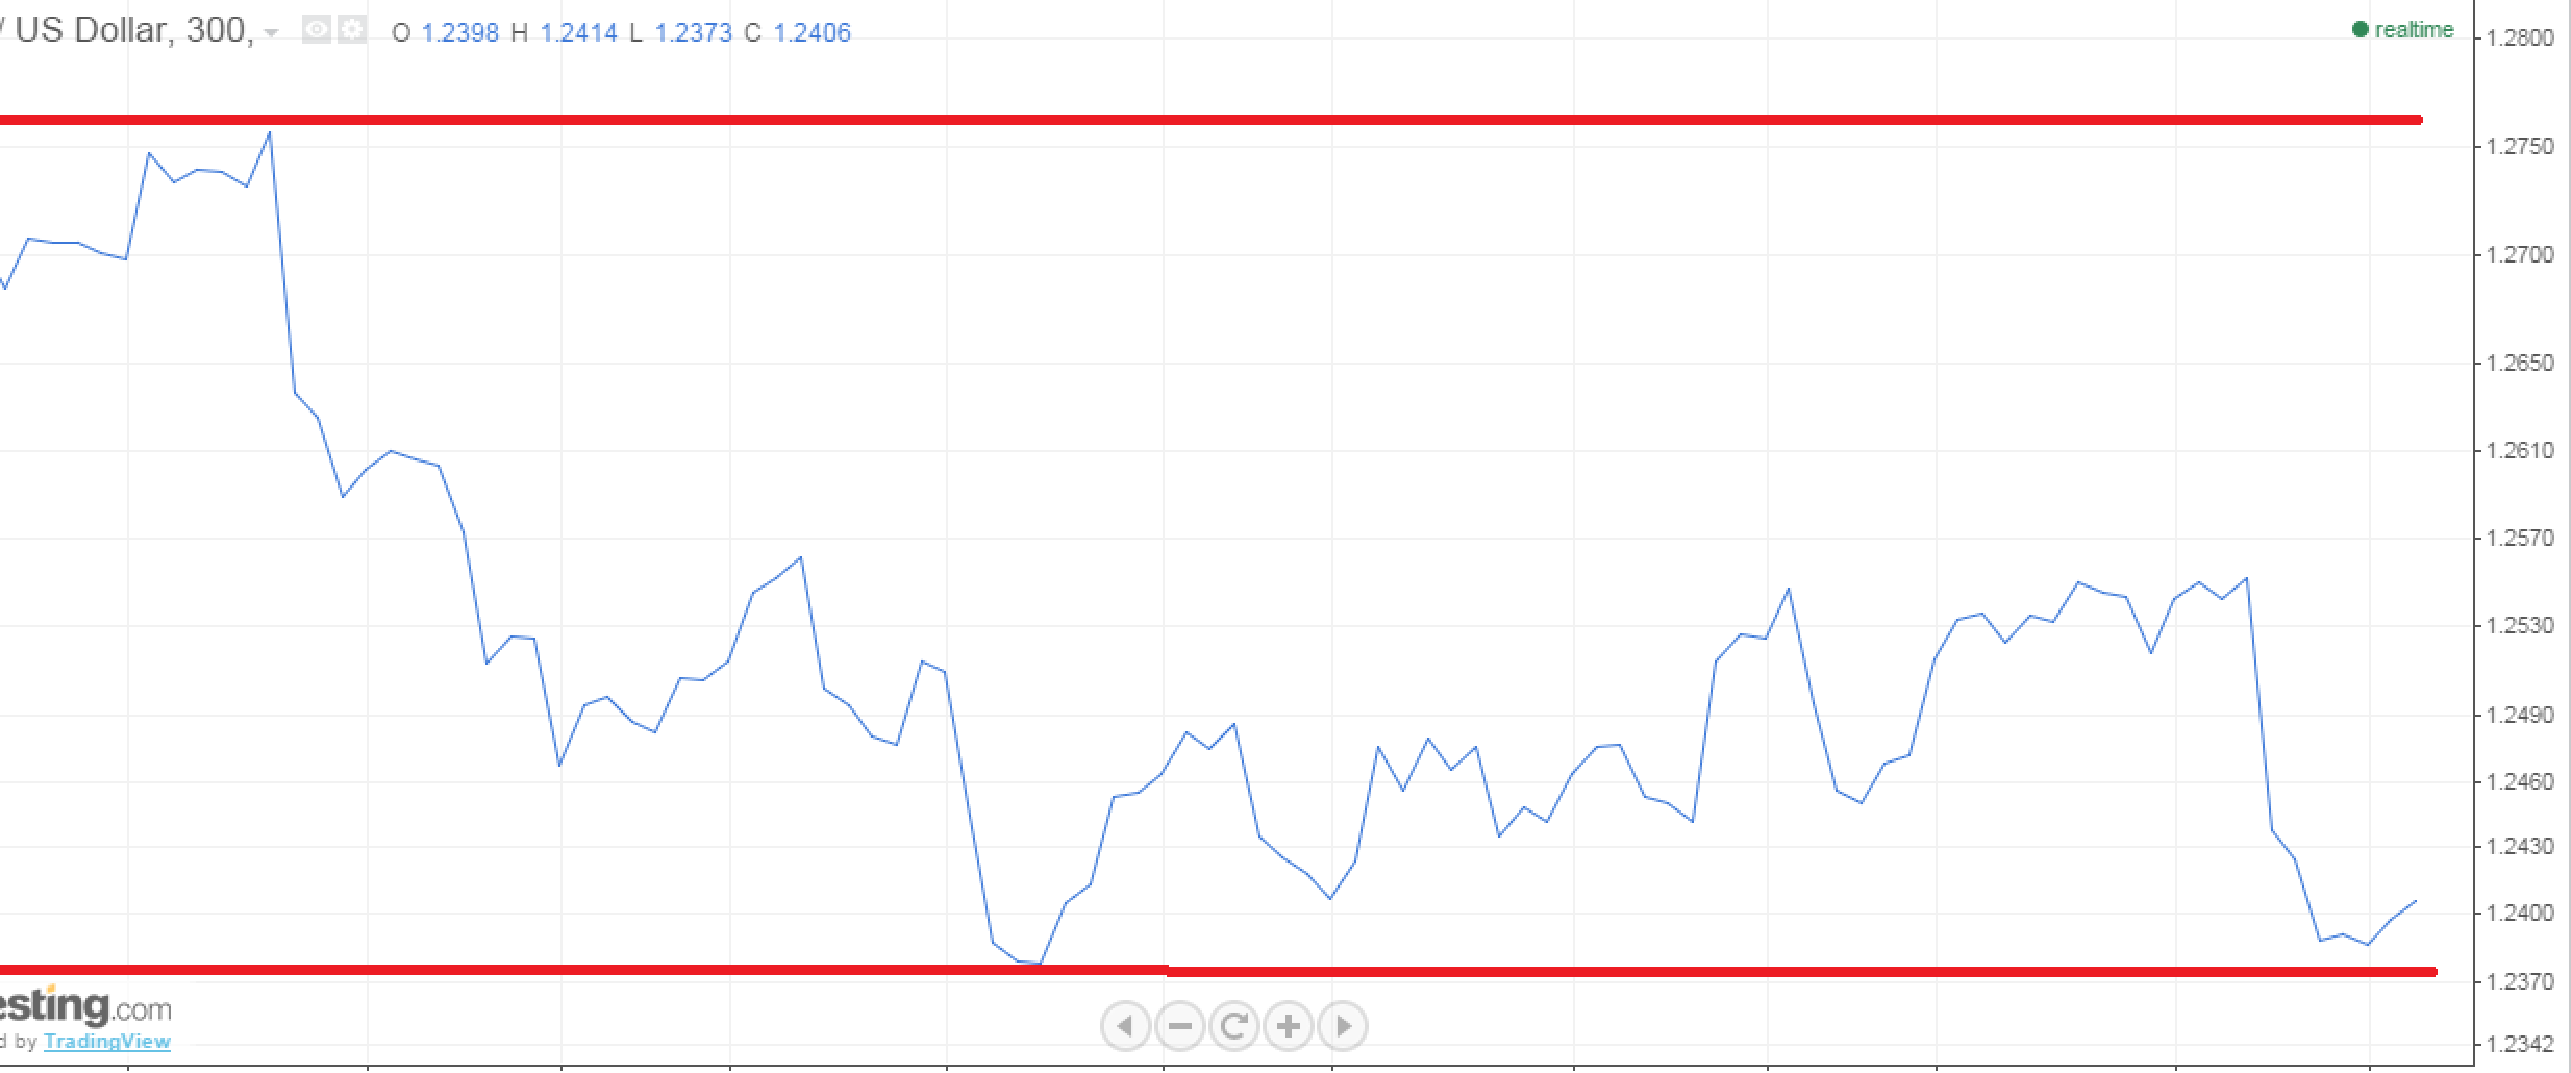
\includegraphics[width=1\textwidth]{obr2} 
Na rozdiel od ďalšej málo volatilnej burzy, kde je  možný zisk iba 2,95 percenta a jeden dielik je tisícina danej meny. 
\subsubsection{Absencia \uv{Veľkých hráčov}} 
Veľký hráči\cite{ZAC} sú hlavne veľké korporácie a bohatí investori. Za to my sme na trhu malí hráči, lebo máme malý kapitál. Ale prečo nie sú na okrajových burzách veľký hráči? Práve preto, že na okrajových burzách sa točí malé množstvo peňazí a na ich investíciách by sa výrazne prejavila likvidita, čo vysvetlím v nevýhodách. 
\subsubsection{Nízke poplatky} 
Keďže máme malý kapitál, ktorý investujeme, veľmi rýchlo by sme skrachovali, keby poplatok za každú transakciu  bol vysoký. Takže veľkou výhodou na okrajových burzách je, že sa dajú nájsť burzy s minimálnymi vstupnými a inými poplatkami. 
\subsection{Nevýhody} 
\subsubsection{Veľká likvidita trhu} 
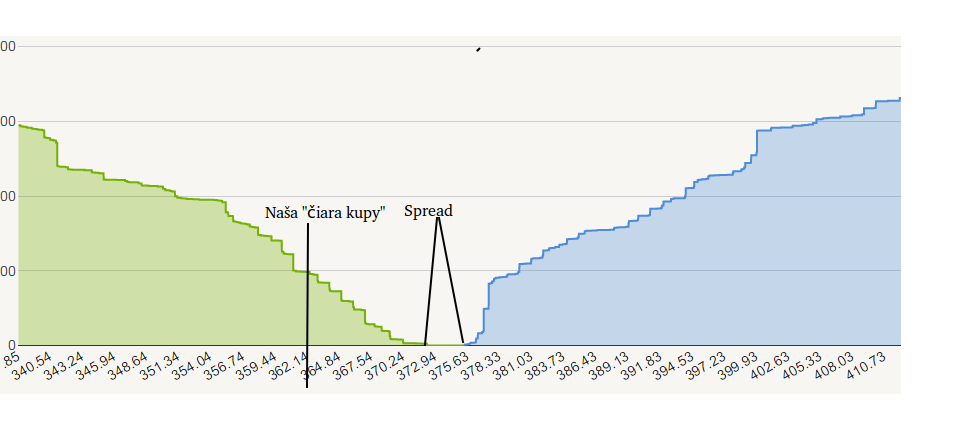
\includegraphics[width=1\textwidth]{stamp} 
Najprv vysvetlím pojem \uv{spread}\cite{ZAC}. Spread je rozdiel medzi ponukou a dopytom. Ak je ponuka 1,5 a dopyt 1,6 spread je 0,1. Likvidita trhu vyjadruje zmenu ceny pri obchodoch. Ak je likvidita vysoká, tak veľké investície zmenia cenu meny a naopak ak je nízka veľké obchody s cenou takmer nič neurobia. Súvisí to stým aké veľké množstvo peňazí sa \uv{točí} na burze. Napríklad pozrime sa na obrázok vyššie. Predstavme si že tento trh ma vysokú likviditu. Na obrázku vidíte ponuku, dopyt a spread. Ak niekto chce spraviť obchod za 1000 dolárov len malé percento zo sumy kúpi za aktuálny kurz zvyšok drahšie až príde po našu čiaru kúpy. Dokým trh nezareaguje vznikne obrovský spread a tiež to zamáva s kurzom. Veľkým hráčom sa neoplatí obchodovať na okrajových burzách, pretože by to pri veľkých investíciach nebolo výhodné. 
\subsubsection{Väčšie riziko} 
Na okrajových burzách je väčšie riziko že svoje investícii stratíš bez tvojho pričinenia. Či sa burza zrazu vyparí za záhadných okolnosti alebo ju niekto \uv{vybrakuje} a už nič nezostane pre teba. Stalo sa v nedávnej minulosti že významné okrajové burzy, zo dňa na deň zmizli a ľudia prišli o svoje investície.  
\subsection{Zhrnutie} 
Z toho čo som vyššie napísal je zjavné,  že pre naše zámery je okrajová burza ideálna. Keďže naše investície do burzy nie sú veľké, veľkou výhodou sú pre nás nízke poplatky a malou nevýhodou vysoká likvidita. Z rizikom že prídeme zo dňa na deň o všetko sa musíme zmieriť. Tiež absencia veľkých hráčov nám vyhovuje, lebo tí by mohli stabilizovať burzu a tým pádom by sme prišli o vysokú volatilitu, ktorá je pre nás výhodou. Ktoré burzy(platformy) vyhovujú našim požiadavkám uvediem ďalej. Ak by sme sa chceli niekedy venovať aj nie okrajovým burzám potrebovali by sme brokera. 
\subsubsection{Broker} 
Je niečo ako investor. Jednak vybaví všetky formality aby sme sa vôbec mohli na takú burzu dostať, lebo to nieje samozrejmosť, a taktiež do nás investuje. Uvediem príklad. My investujeme povedzme 1000 dolárov a on nakoniec pridá dve nuly, takže pochopiteľne nám to zvýši výnos, z ktorého si broker berie nemalú časť. Samozrejme broker dáva pozor aby sme nestratili jeho peniaze a ak by sme mali klesnúť pod hranicu jeho peňazí zakáže nám ďalej obchodovať.\cite{ZAC} 
\section{Vyhovujúce platformy} 
Ďalšou s vecí ktoré potrebuje aby mala naša burza, a ešte som to nespomenul, je aby mala API. To znamená že povoľuje aby s nou mohol pracovať náš algoritmus. V tejto časti si predstavíme burzy ktoré najviac vyhovujú naším požiadavkám. Sú to všetko burzy so pseudo-menami a hlavne s bitcoinom, lebo ten má pre nás veľmi dobré vlastnosti. 
\subsubsection{BITSTAMP} 
Túto burzu preferujeme najviac a na tejto burze chceme začať. Moja bakalárka sa bude týkať asi hlavne tejto burzy. BITSTAMP ma veľmi prehľadné API, vyhovujúce transakčné poplatky a iné nám potrebné vlastnosti. Transakčné poplatky sú od 0,5 percenta z transakcie, keď je transakcia do 500 dolárov až po 0,2 percenta keď je naša transakcia nad 120000 dolárov. Obchodovaní pár je BTC/USD. \cite{Bit} 
\subsubsection{Bitfinex} 
Tu sa poplatky pohybujú od 0,1 až po 0,2 percenta z transakcie. Obchodovaní pár je BTC/USD. Okrem bitcoinu sa dá obchodovať ešte z namecoinom a litecoinom. \cite{Bitf} 
\subsubsection{BTC-e} 
Poplatky sa transakciu sú od 0,2 do 0,5. Obchodovaní pár je BTC/USD. \cite{BTC} 
\subsubsection{Kraken} 
Táto burza okrem bitcoinu obchoduje s viac inými pseudo-menami, preto túto burzu by sme použili keby sme chceli prejsť na tieto meny. \cite{Kre} 
\section{Existujúce riešenie} 
\subsection{Tradewave} 
Toto existujúce riešenie vzniklo iba toto leto, tým pádom až potom ako sme začali rozvíjať našu myšlienku. Tradewave je veľmi podobný tomu čo chceme my robiť, ba priam v užívateľskom rozhraní je ešte lepší ale je tu jedna veľká nevýhoda kvôli čomu nemôžme Tradewave použiť.  
\subsubsection{Čo je to Tradevawe?}
Tradewave je veľmi pohodlní spôsob ako si vytvoriť vlastní obchodovací algoritmus. Programátorský jazyk sa používa Python. Obchoduje práve na tých platformách, ktoré som spomínal v časti \uv{Vyhovujúce platformy}. Je kompletne automatizovaný. Obchody grafy a záznamy zobrazuje v reálnom čase. Algoritmus môže bežať neustále na ich serveroch a tiež sa pohodlne spustiť a zastaviť. Dokonca a aj mailové upozorňovanie. Na ich stránke sa dá váš algoritmus aj jednoducho rýchlo testovať na historických dátach.  \cite{Tw} 
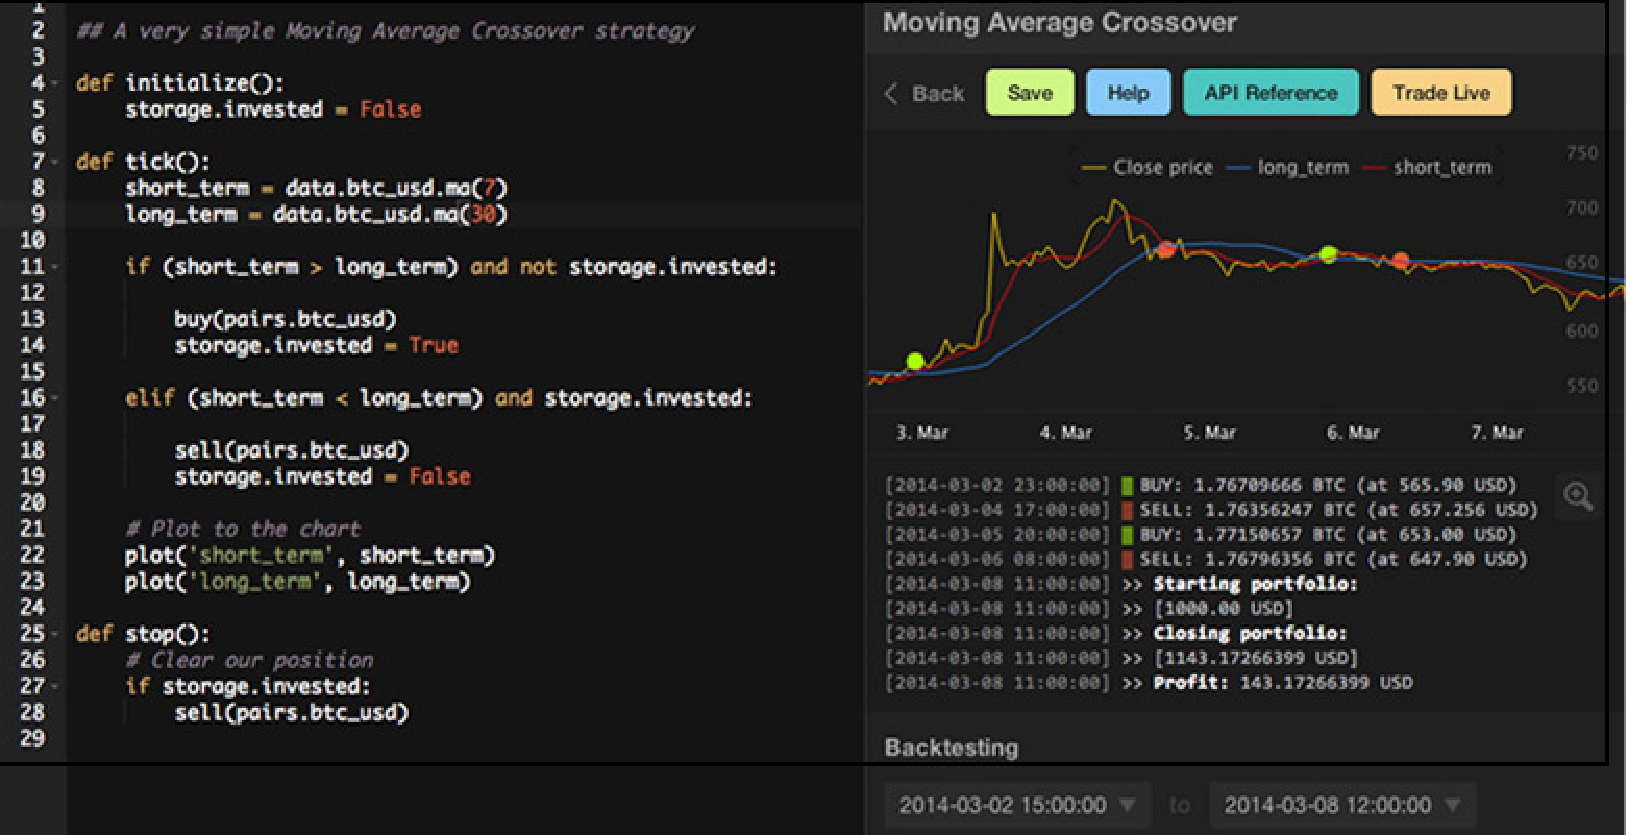
\includegraphics[width=1\textwidth]{trade} 
\subsubsection{Čo vzhľadom ku nám?}
Toto riešenie je oproti nám veľmi užívateľský pohodlné. My sa nebudeme venovať užívateľskému rozhraniu, keďže budeme z naším algoritmom a testovaním  pracovať iba my. Ale bohužiaľ nebudeme môcť použiť nič z tohto existujúceho riešenia jednak nie sú verejné kódy a druhá vec, čo je hlavný dôvod prečo nemôžme Tradewave použiť, je že pri používaní tejto platformy sa stáva tvoj kód ich kódom. Tvoj nápad ich nápadom. To je aj dôvod že používanie Tradewave je zadarmo. Vzhľadom na to že v budúcnosti by sme chceli na našom algoritme aj zarábať nemôžme si dovoliť použiť Tradewave a tak odovzdať naše nápady, dokonca už aj naprogramované, niekomu inému.
\section{Použité technológie} 
V tejto časti predstavím sú technológie ktoré budú použité pri programovaní algoritmu a testovania.
\subsubsection{Ruby}
Väčšina kódu bude naprogramovaná jazyku v Ruby. Ruby je dynamický, open source programovací jazyk so zameraním na jednoduchosť a produktivitu. Má elegantnú syntax, ktorú je prirodzené čítať a jednoduché písať. Ruby bol prvý krát uvedený v roku 1995 svojím tvorcom Yukihiro “Matz” Matsumoto. Matz skombinoval svoje obľúbené jazyky (Perl, Smalltalk, Eiffel, Ada, and Lisp). Ruby je vyvážením funkcionálneho a imperatívneho programovania. Svojej obľube sa teší až od roku 2006.\cite{Rb} 
\subsubsection{Python} 
Nejaké časti kódu sa môžu objaviť aj v jazyku Python. Python je interpretovaný, objektovo orientovaný, vysoko-úrovňoví programovací jazyk s dynamickou sémantikou. Je postavený na dátových štruktúrach, v kombinácii s dynamickým písaním a dynamickými väzbami, aby bol atraktívny pre rýchly vývoj aplikácií. Rovnako použitý ako skriptovací jazyk alebo \uv{lepidlo} jazyk na pripojenie existujúcich komponentov dohromady. Prvé uvedenie Pythonu je z decembra 1989 svojím tvorcom Guido van Rossum\cite{Pt} 
\section{Bitcoin} 
V poslednej časti úvodnej kapitoly predstavím pseudo-menu bitcoin. Dávam ju do pozornosti preto, lebo práve trhy kde sa obchoduje s bitcoinami, majú pre nás vyhovujúce vlastnosti a preto bude náš obchodovací pár vždy v spojení s bitcoinom.
\subsection{O bitcoine} 
Bitcoin umožňuje nový platobný systém s úplne digitálnymi peniazmi. Jedná sa o prvú decentralizovaná platbu siete peer-to-peer, ktorý je poháňaná svojim užívateľom bez ústredného orgánu alebo sprostredkovateľov. Z užívateľského hľadiska je bitcoin skoro ako prevodom cez internet. Bitcoin je prvá realizácia koncepcie nazvanej \uv{krypto meny}, ktorá bola prvýkrát popísaná v roku 1998 Wei Dai v \uv{cypherpunks} mailovom zozname, čo naznačovala myšlienku novej formy peňazí, ktorá používa šifrovanie na riadenie jej vzniku a transakcií, miesto centrálnych autorít.  Prvá špecifikácia bola publikovaná v roku 2009  Satoshi Nakamotom. 
\subsection{Spôsob získavania}
Bitcoini môžete získať buď že vám niekto nimi zaplatí, že ich kúpite na burze alebo ich dostanete. Ale existuje ešte jeden zaujímavý spôsob a to je ťažba.
\subsubsection{Ťažba}
Toto je spôsob keď požičiate svoju výpočtovou silu na vedecké účeli, čím viac tým lepšie, a takýmto spôsobom môžete ťažiť bitcoin.
\subsection{Použitie}
Bitcoin sa v hojnej miere používa už na internete. Podporuje ho už aj veľa známych obchodov. Bohužiaľ keďže bitcoin je slabo od kontrolovateľný,
 často sa využíva na nelegálne obchody s drogami alebo na pranie peňazí. Dokonca niektoré ne-internetové obchody zaviedli platenie bitcoinami. Na Slovensku máme už aj bitcoinoví bankomat. 
\cite{B} 
